\documentclass[12pt,a4paper]{ctexart}

% =========================
% Packages
% =========================
\usepackage[a4paper,margin=2.35cm]{geometry}
\usepackage{setspace}
\usepackage{amsmath,amssymb,bm}
\usepackage{booktabs,array,multirow,longtable}
\usepackage{graphicx}
\usepackage{float}
\usepackage{caption}
\usepackage{subcaption}
\usepackage{enumitem}
\usepackage{hyperref}
\usepackage{xcolor}
\usepackage{fancyhdr}
\usepackage{titlesec}
\usepackage{tocloft}
\usepackage{threeparttable}
\usepackage{pdflscape}

% =========================
% Hyperref
% =========================
\hypersetup{
    colorlinks=true,
    linkcolor=black,
    citecolor=black,
    urlcolor=blue,
    pdftitle={基于宏观状态调整的风险预算资产配置模型研究},
    pdfauthor={Putian Zhao},
    pdfsubject={Multi-Asset Allocation, Risk Budgeting, Macro Regime},
    pdfkeywords={风险预算, 风险平价, 宏观配置, 多资产配置, ETF}
}

% =========================
% Spacing & Style
% =========================
\setstretch{1.28}
\captionsetup{font=small,labelsep=space}
\setlength{\parskip}{0.45em}
\setlength{\parindent}{2em}

\titleformat{\section}{\bfseries\Large}{\thesection}{0.8em}{}
\titleformat{\subsection}{\bfseries\large}{\thesubsection}{0.8em}{}
\titleformat{\subsubsection}{\bfseries\normalsize}{\thesubsubsection}{0.8em}{}

\pagestyle{fancy}
\fancyhf{}
\fancyhead[L]{基于宏观状态调整的风险预算资产配置模型研究}
\fancyhead[R]{\thepage}

% =========================
% Custom Commands
% =========================
\newcommand{\HRule}{\rule{\linewidth}{0.5mm}}
\newcommand{\note}[1]{\textcolor{gray}{\small #1}}

% =========================
% Document
% =========================
\begin{document}

% =========================
% Cover
% =========================
\begin{titlepage}
    \centering
    \vspace*{2.2cm}

    {\zihao{2}\bfseries 多资产量化配置策略构建与绩效评估\par}
    \vspace{1.2cm}

    {\zihao{4}课题研究报告\par}
    \vspace{0.8cm}

    {\large FICC买方实习生\ 赵浦添\par}
    \vspace{0.5cm}
    {\large \today\par}

    \vfill

    \begin{minipage}{0.86\textwidth}
    \setstretch{1.4}
    \zihao{-4}
    本报告围绕多资产配置中的风险预算框架展开，构建基准风险平价组合与宏观驱动稳定版组合，并对其在历史样本与验证样本中的收益、波动、回撤、换手与资产集中度进行比较。研究重点不在于“拍脑袋择时”，而在于将宏观信息作为风险预算调节器嵌入配置引擎，在协方差结构仍主导最终权重映射的前提下，提升组合对经济状态变化的响应能力。
    \end{minipage}

    \vfill
\end{titlepage}

\tableofcontents
\newpage

% =========================
\section{摘要}
% =========================

随着多资产配置策略在机构投资中的广泛应用，风险平价（Risk Parity）与风险预算（Risk Budgeting）方法已成为构建稳健组合的重要工具。传统风险平价框架的优点在于弱化了对预期收益率的依赖，但其配置逻辑主要建立在历史协方差结构之上，对宏观环境变化的适应性相对有限。若市场所处经济阶段发生切换，仅依赖过去波动与相关性进行配置，往往容易在组合风险暴露上出现“后知后觉”的问题。

基于这一现实动机，本文在传统风险预算框架之上，引入宏观经济信号，对资产层面的风险预算进行动态调整，构建宏观驱动的稳定版多资产配置模型（Macro Stable）。在该模型中，宏观信号不直接指定最终持仓权重，而是先作用于风险预算，再由协方差结构将预算映射为资产权重。换言之，宏观变量扮演的是“方向盘”而不是“油门”，最终车轮的转角仍然由组合风险结构决定。这一设计既保留了风险平价框架的稳定性，也引入了对经济状态切换的响应能力。

本文的资产池包含六类资产：沪深300、标普500、10年期国债、黄金、政策性金融债与信用债。研究采用日度收益率数据、月度调仓、252个交易日滚动窗口与5\%目标波动率设定，构建Baseline风险平价策略与Macro Stable宏观稳定版策略，并从回测段（2018--2023）与验证段（2024--2025）两个维度比较绩效。代码实现显示，基准策略使用SLSQP求解等风险贡献权重，并在目标波动率约束下自动生成现金仓位；宏观稳定版则在风险预算基础上依次叠加单资产上限、单次权重变化限制、目标波动率缩放与最低现金比例约束，风控链条更完整、更贴近机构实务。

结果显示，在回测段中，Macro Stable相较Baseline收益略高，但波动率与回撤也更高；而在验证段中，Macro Stable取得了更高的年化收益（6.77\% vs. 5.11\%）、更低的年化波动（4.44\% vs. 4.71\%）以及更浅的最大回撤（-5.47\% vs. -6.65\%），验证期Sharpe比率也显著占优。与此同时，Macro Stable的平均现金比例更高（15.39\% vs. 4.60\%），最大单资产权重更低（38.83\% vs. 59.46\%），但月度平均换手率更高（8.92\% vs. 3.82\%）。这些结果表明，宏观风险预算机制在提升组合防御性和结构分散度方面具有明显作用，但也以更高的调仓频率为代价。上述结果与模型摘要中给出的自动输出指标一致。

总体而言，本文的研究结论是：在风险预算框架下引入宏观信息并不意味着放弃风险平价，而是让风险平价从“静态均衡”向“条件均衡”迈进一步。宏观信号不是替代协方差，而是为协方差提供状态上下文。对机构投资而言，这种思路具有较强的解释性、可扩展性与实操价值。

\newpage

% =========================
\section{研究背景与问题提出}
% =========================

资产配置始终是投资管理中的核心命题。传统均值--方差框架通过预期收益、波动率与协方差三者联合优化，为现代组合理论奠定了基础。然而，在真实投资场景中，预期收益往往最难估、也最容易估错。收益预测稍有偏差，最优权重就可能出现明显扭曲，因此许多机构投资者在长期实践中逐渐转向对收益假设更不敏感的配置框架。

风险平价与风险预算正是在这样的背景下获得广泛应用。其核心逻辑不是让资金均分，而是让风险更均匀地分配到各类资产上。对于债券、权益、黄金、信用等波动特征差异显著的资产而言，这一方法能够避免传统市值加权或简单等权重组合中常见的“表面分散、实则单一风险源占主导”的问题。

但风险平价也并非没有盲区。它擅长处理“已发生过的风险结构”，却未必天然擅长处理“正在发生变化的宏观环境”。当经济由复苏转入过热，由紧缩转入放松，或由扩张切换至放缓时，资产未来一段时间的相对表现与历史关系往往会出现变化。如果组合仍仅根据历史协方差均匀分配风险，配置结果可能在时点上偏慢，在状态上偏钝。

因此，本文希望回答以下问题：

\begin{enumerate}[label=\arabic*)]
    \item 在风险预算框架中引入宏观信号，是否能够提升多资产组合的配置表现？
    \item 如果宏观信息只用于调整风险预算，而不直接决定最终权重，能否同时兼顾模型稳定性与状态响应能力？
    \item 在收益、回撤、波动、换手率、现金仓位与集中度之间，Macro Stable相较Baseline呈现出何种权衡关系？
\end{enumerate}

这三个问题共同构成本文研究的主线。用更直白的话说，本文不是要做一个“激进择时模型”，而是试图搭一座桥，把宏观信息稳稳地接到风险预算引擎上，让组合在不失控的前提下，具备更强的状态感知能力。

% =========================
\section{数据说明与资产池构建}
% =========================

\subsection{资产池选择}

本文最终采用六类资产构建组合，分别为：

\begin{enumerate}[label=\arabic*)]
    \item 沪深300（hs300）
    \item 标普500（sp500）
    \item 10年期国债（cgb10y）
    \item 黄金（gold）
    \item 政策性金融债（policy\_bond）
    \item 信用债（credit\_bond）
\end{enumerate}

从代码实现看，资产价格面板由上述六类资产组成，且样本起点统一截取为2016年1月4日。这一资产池具备较好的代表性：权益资产对应经济增长弹性，利率债与政策债提供防御性与利率敏感暴露，黄金作为典型避险及通胀对冲资产，信用债则引入票息与信用利差维度。六者共同构成了一套较为完整的多资产风险拼图。

\subsection{数据衔接与价格面板构造}

在真实市场数据处理中，ETF历史长度往往不足以覆盖完整研究期，因此本文采用“ETF优先、指数回补”的方式构建连续价格序列。其中，10年期国债与政策性金融债资产均通过指数收益对ETF历史进行回补；信用债资产则更具特殊性，其构造方式为：2022年7月1日至2025年1月21日使用信用债指数，2025年1月22日起切换为511070 ETF实盘价格。这意味着信用债资产在样本前段存在覆盖区间限制，也解释了为何后续结果中某些年份的资产集中与波动表现会呈现阶段性特征。

从研究方法上讲，这样的数据拼接方式并不完美，但它在课题实务中是合理且必要的。因为机构研究常面对一个朴素而尖锐的问题：如果只保留“完美覆盖”的资产，研究区间就会被压缩得很短；如果完全放弃可交易ETF，只使用长历史指数，则又会削弱结果的投资可落地性。本文采取的方式，正是在“历史长度”与“投资可实现性”之间做平衡。

\subsection{收益率与宏观面板}

资产收益率面板基于价格序列计算得到，研究主回测文件使用 \texttt{asset\_return\_panel.csv}。宏观面板则包含至少三个变量：PMI、CPI与CN10Y，在宏观稳定版回测加载环节中被明确读取。这三个变量分别对应增长、通胀与利率环境，构成最基础也最容易解释的宏观三维结构。

在我看来，这个宏观变量组合的优点在于它不花哨。它不是为了堆砌“高级感”而塞进一串难以解释的黑箱因子，而是选择了最能和资产收益方向产生明确映射关系的几个核心维度。这样做的好处是，无论写论文、做答辩还是面对投资经理追问，模型逻辑都不容易散架。

% =========================
\section{模型框架与方法设计}
% =========================

\subsection{Baseline：基准风险平价模型}

基准模型采用典型风险平价思想。设资产权重向量为
\[
\bm{w} = (w_1,w_2,\dots,w_N)^\top,
\]
协方差矩阵为
\[
\Sigma.
\]
则组合方差为
\[
\sigma_p^2 = \bm{w}^\top \Sigma \bm{w},
\]
组合波动率为
\[
\sigma_p = \sqrt{\bm{w}^\top \Sigma \bm{w}}.
\]

对第 \(i\) 个资产，其边际风险贡献为
\[
MRC_i = (\Sigma \bm{w})_i,
\]
风险贡献可写为
\[
RC_i = w_i(\Sigma \bm{w})_i.
\]

在Baseline模型中，目标是让各资产风险贡献占比尽量接近均等，即
\[
\frac{RC_i}{\sum_{j=1}^{N} RC_j} \approx \frac{1}{N}, \quad i=1,2,\dots,N.
\]

从代码实现看，Baseline使用SLSQP优化器，在权重和为1、单资产权重位于0到1之间的约束下求解风险平价权重。目标函数本质上是最小化风险贡献占比与等权风险目标之间的偏差平方和。也就是说，Baseline不是简单的等资金配置，而是追求等风险配置。

\subsection{波动率目标与现金头寸}

Baseline模型得到风险平价权重后，并不直接满仓持有，而是进一步通过目标波动率机制决定是否缩放风险资产权重。代码中将目标波动率设为5\%，若组合年化波动率高于该水平，则按比例缩小风险资产敞口，并将剩余权重配置为现金。目标波动率5\%这一设定在展示摘要中也被明确说明。

这一步很关键。它相当于给组合装上了一个“保险丝”，当风险结构变得躁动时，组合不会被迫满仓硬扛，而是可以通过抬升现金比例降低总波动暴露。

\subsection{平滑机制}

Baseline回测中还加入了权重平滑机制。若上一个调仓期已有有效权重，则当前新权重不会被完全采用，而是按
\[
w_t^{final} = 0.7 w_{t-1}^{final} + 0.3 w_t^{new}
\]
进行平滑过渡。这一设定降低了权重突变，也在一定程度上抑制了交易冲击和信号噪声。机构视角下，这一步很像给模型加了减震器，避免组合像踩到井盖一样一跳一跳。

\subsection{Macro Stable：宏观驱动稳定版模型}

Macro Stable模型延续风险预算框架，但不再将所有资产的风险预算固定为均等，而是根据宏观状态动态调整预算。其核心顺序在代码中非常清楚：

\begin{enumerate}[label=\arabic*)]
    \item 识别宏观状态；
    \item 调整基础风险预算；
    \item 求解风险预算权重；
    \item 施加单资产权重上限；
    \item 施加单次权重变化限制；
    \item 进行目标波动率缩放；
    \item 施加最低现金比例约束。
\end{enumerate}

上述流程在宏观稳定版引擎中被逐步实现。对应的求解器不是SLSQP，而是一个自定义迭代法，其思路是不断调整权重，使风险贡献占比逼近给定的风险预算向量。

这和Baseline最大的不同在于：Baseline追求“每个人都分到一样大的风险蛋糕”，Macro Stable则允许在宏观状态切换时，某些资产分到更大的那一块，但蛋糕怎么切，依然要服从协方差矩阵这位“总管家”的秩序。

\subsection{宏观信号的角色}

展示摘要里对这一点表述得非常准确：宏观版本中，宏观信号仅用于调整风险预算，最终权重仍通过协方差结构映射得到。这句话几乎就是整篇课题最该被记住的一句话。

从研究设计上，这种做法比“宏观信号直接改权重”更稳健，原因有三：

\begin{enumerate}[label=\arabic*)]
    \item 宏观信息通常方向感较强，但精确到具体权重并不可靠；
    \item 协方差结构仍保留了资产间联动与风险分散信息；
    \item 模型解释上更自然，能说清楚“宏观因子到底改了什么”。
\end{enumerate}

因此，Macro Stable的本质不是“宏观择时模型”，而是“宏观调节下的动态风险预算模型”。

% =========================
\section{回测设计与绩效指标}
% =========================

\subsection{调仓频率与样本窗口}

两类策略均采用月度调仓框架，调仓日被识别为每月最后一个交易日。协方差矩阵估计窗口为252个交易日，对应约1年滚动历史长度。这一设定兼顾了样本稳定性与状态敏感度，避免使用过短窗口引起协方差估计大幅抖动，也避免过长窗口让风险结构反应变慢。

\subsection{绩效指标}

本文使用以下指标评价组合表现：

\begin{enumerate}[label=\arabic*)]
    \item 年化收益率（Annual Return）
    \item 年化波动率（Annual Volatility）
    \item Sharpe比率
    \item 最大回撤（Max Drawdown）
    \item Calmar比率
\end{enumerate}

相关计算方法在Baseline与Macro Stable引擎中基本一致，均基于组合收益序列计算累计净值、波动率和最大回撤。

此外，考虑到机构配置更关心组合可交易性与风控稳健性，本文还跟踪了以下结构性指标：

\begin{enumerate}[label=\arabic*)]
    \item 平均现金比例
    \item 最大单资产权重
    \item 最大单次权重变化
    \item 月度平均换手率
\end{enumerate}

这些指标在展示摘要中均有明确输出。

% =========================
\section{实证结果分析}
% =========================

\subsection{总体绩效对比}

根据自动生成的结果摘要，在回测段（2018--2023）中，Baseline策略年化收益率为4.25\%，年化波动率为2.78\%，Sharpe比率为1.529，最大回撤为-3.27\%；Macro Stable策略年化收益率为4.54\%，年化波动率为3.99\%，Sharpe比率为1.137，最大回撤为-6.12\%。

这意味着在样本内阶段，Macro Stable虽然在收益上略有提升，但代价是波动和回撤都更高。从研究视角看，这种现象并不奇怪。宏观信号加入之后，风险预算不再永远均匀，组合在某些阶段会更明显地向宏观判断偏好的资产倾斜，于是状态响应能力提高了，风险分布也更有“棱角”了。

真正值得关注的是验证段（2024--2025）的表现。该阶段中，Baseline策略年化收益率为5.11\%，年化波动率为4.71\%，Sharpe比率为1.086，最大回撤为-6.65\%；Macro Stable策略年化收益率为6.77\%，年化波动率为4.44\%，Sharpe比率为1.527，最大回撤为-5.47\%。

也就是说，到了样本外验证阶段，Macro Stable不仅跑得更快，而且步子还更稳。对一个资产配置模型来说，这比样本内“过于漂亮”的表现更有说服力。

\subsection{结构性风控指标}

在结构性指标方面，Macro Stable表现出更强的防御性与更低的集中度：

\begin{itemize}
    \item 平均现金比例：15.39\% vs. 4.60\%
    \item 最大单资产权重：38.83\% vs. 59.46\%
    \item 最大单次权重变化：20.16\% vs. 24.62\%
    \item 月度平均换手率：8.92\% vs. 3.82\%
\end{itemize}

上述指标均来自自动摘要输出。

这组数字很有意思。Macro Stable一方面提高了现金比例、压低了单资产集中度，还控制了最大单次权重跳变；但另一方面，它的平均换手率明显更高。这说明宏观稳定版不是“更保守就一定更不动”，而是“更有纪律地动”。它该缩的时候缩，该调的时候调，因此整体风格更像一位谨慎但并不僵硬的组合经理。

\subsection{逐年绩效观察}

从年度绩效图可见，Macro Stable在多数关键年份相对Baseline取得了更优或不弱的收益表现，尤其在2019、2020、2023、2024、2025年均体现出较明显优势；但在2018与2022这类环境较为复杂或信号不占优的年份，其超额收益并非线性稳定存在。

这也提示了一个很真实的结论：宏观预算调整不是魔法，不会在每一年都无条件赢。它的价值更像是让组合在“该看天色的时候看天色”，而不是永远蒙着眼睛按旧地图走路。

% =========================
\section{图形结果与经济解释}
% =========================

\subsection{净值与回撤}

从净值比较图来看，Macro Stable在中后段逐渐拉开与Baseline的净值差距，尤其在验证段体现出更强的累计增值能力。对应地，回撤图显示Macro Stable虽然在个别年份曾出现较深回撤，但在2024--2025验证阶段整体最大回撤控制优于Baseline。结合指标表，这一现象与验证段的风险收益改善相一致。

\begin{figure}[H]
    \centering
    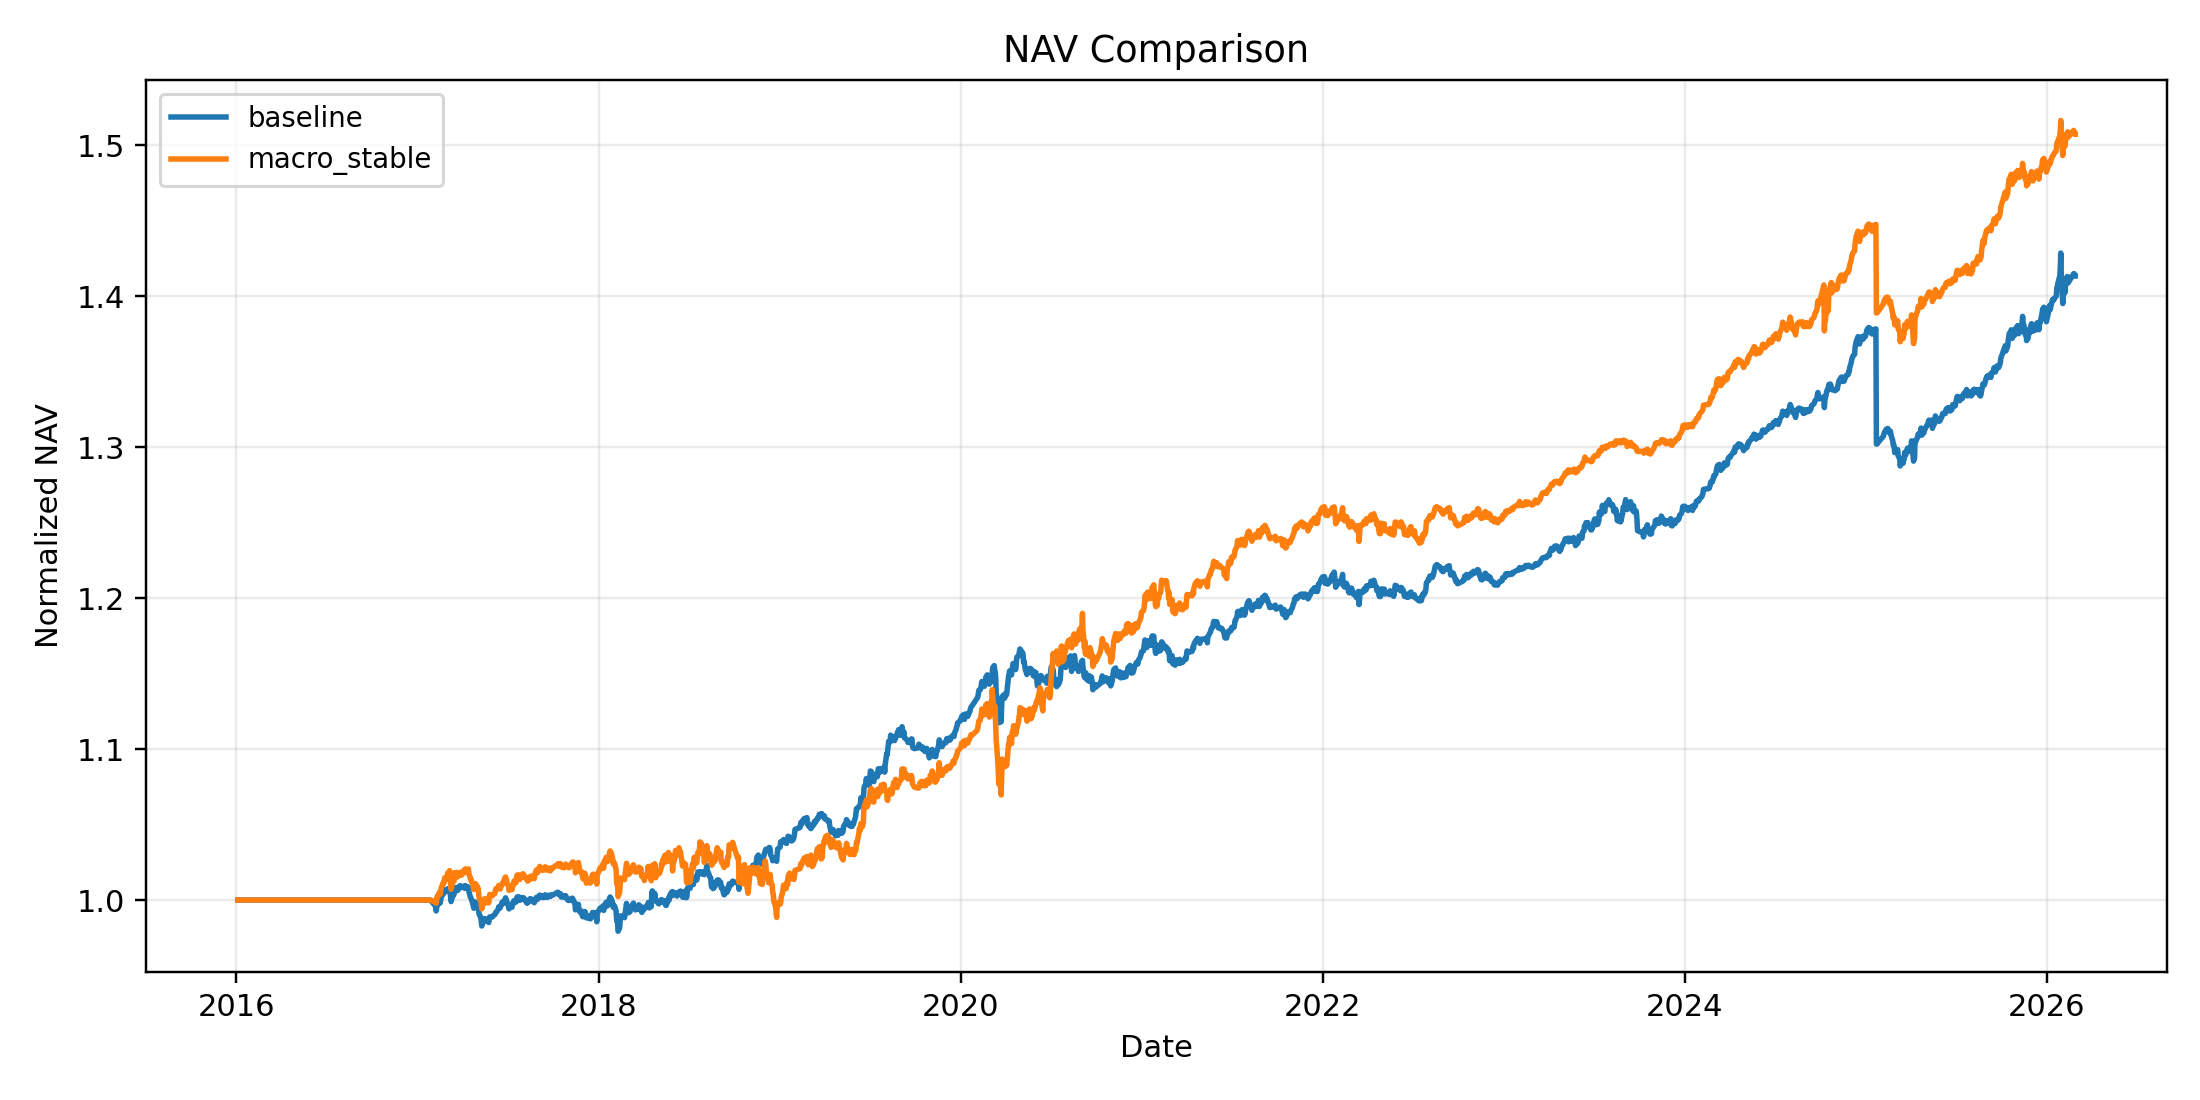
\includegraphics[width=0.88\textwidth]{showcase_output/figures/nav_comparison.png}
    \caption{Baseline 与 Macro Stable 净值曲线对比}
\end{figure}

\begin{figure}[H]
    \centering
    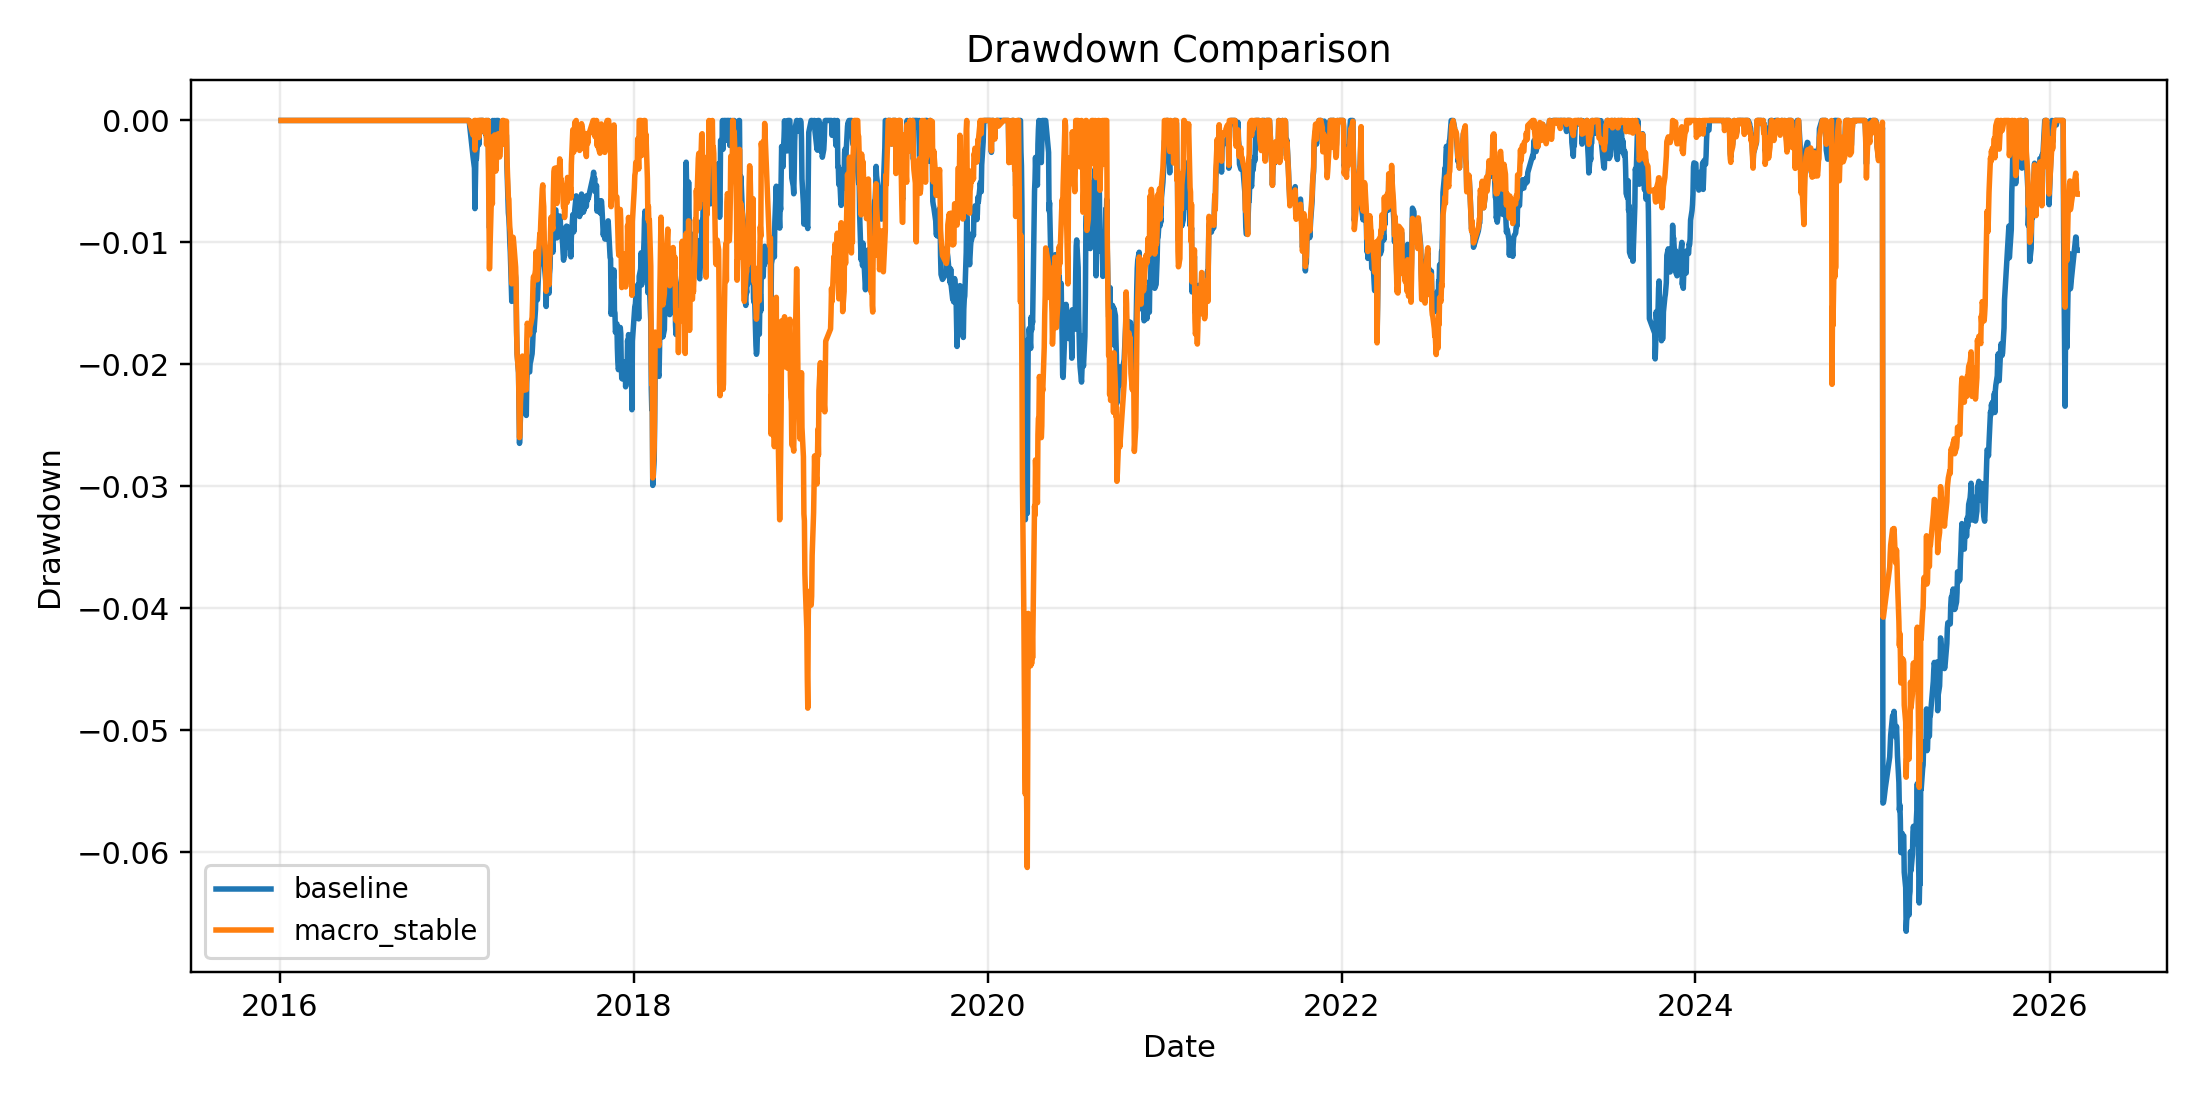
\includegraphics[width=0.88\textwidth]{showcase_output/figures/drawdown_comparison.png}
    \caption{Baseline 与 Macro Stable 回撤曲线对比}
\end{figure}

\subsection{滚动波动率与目标波动率机制}

滚动252日年化波动率图展示了两类策略在不同阶段的风险水平。摘要中明确指出，TARGET\_VOL设定为5\%，作为滚动波动率的展示参照线。从图上看，Macro Stable在若干阶段接近或略高于目标线，但整体验证段波动率水平优于Baseline。结合代码中的目标波动率缩放函数可知，现金仓位的引入是控制总体组合风险的重要来源。

\begin{figure}[H]
    \centering
    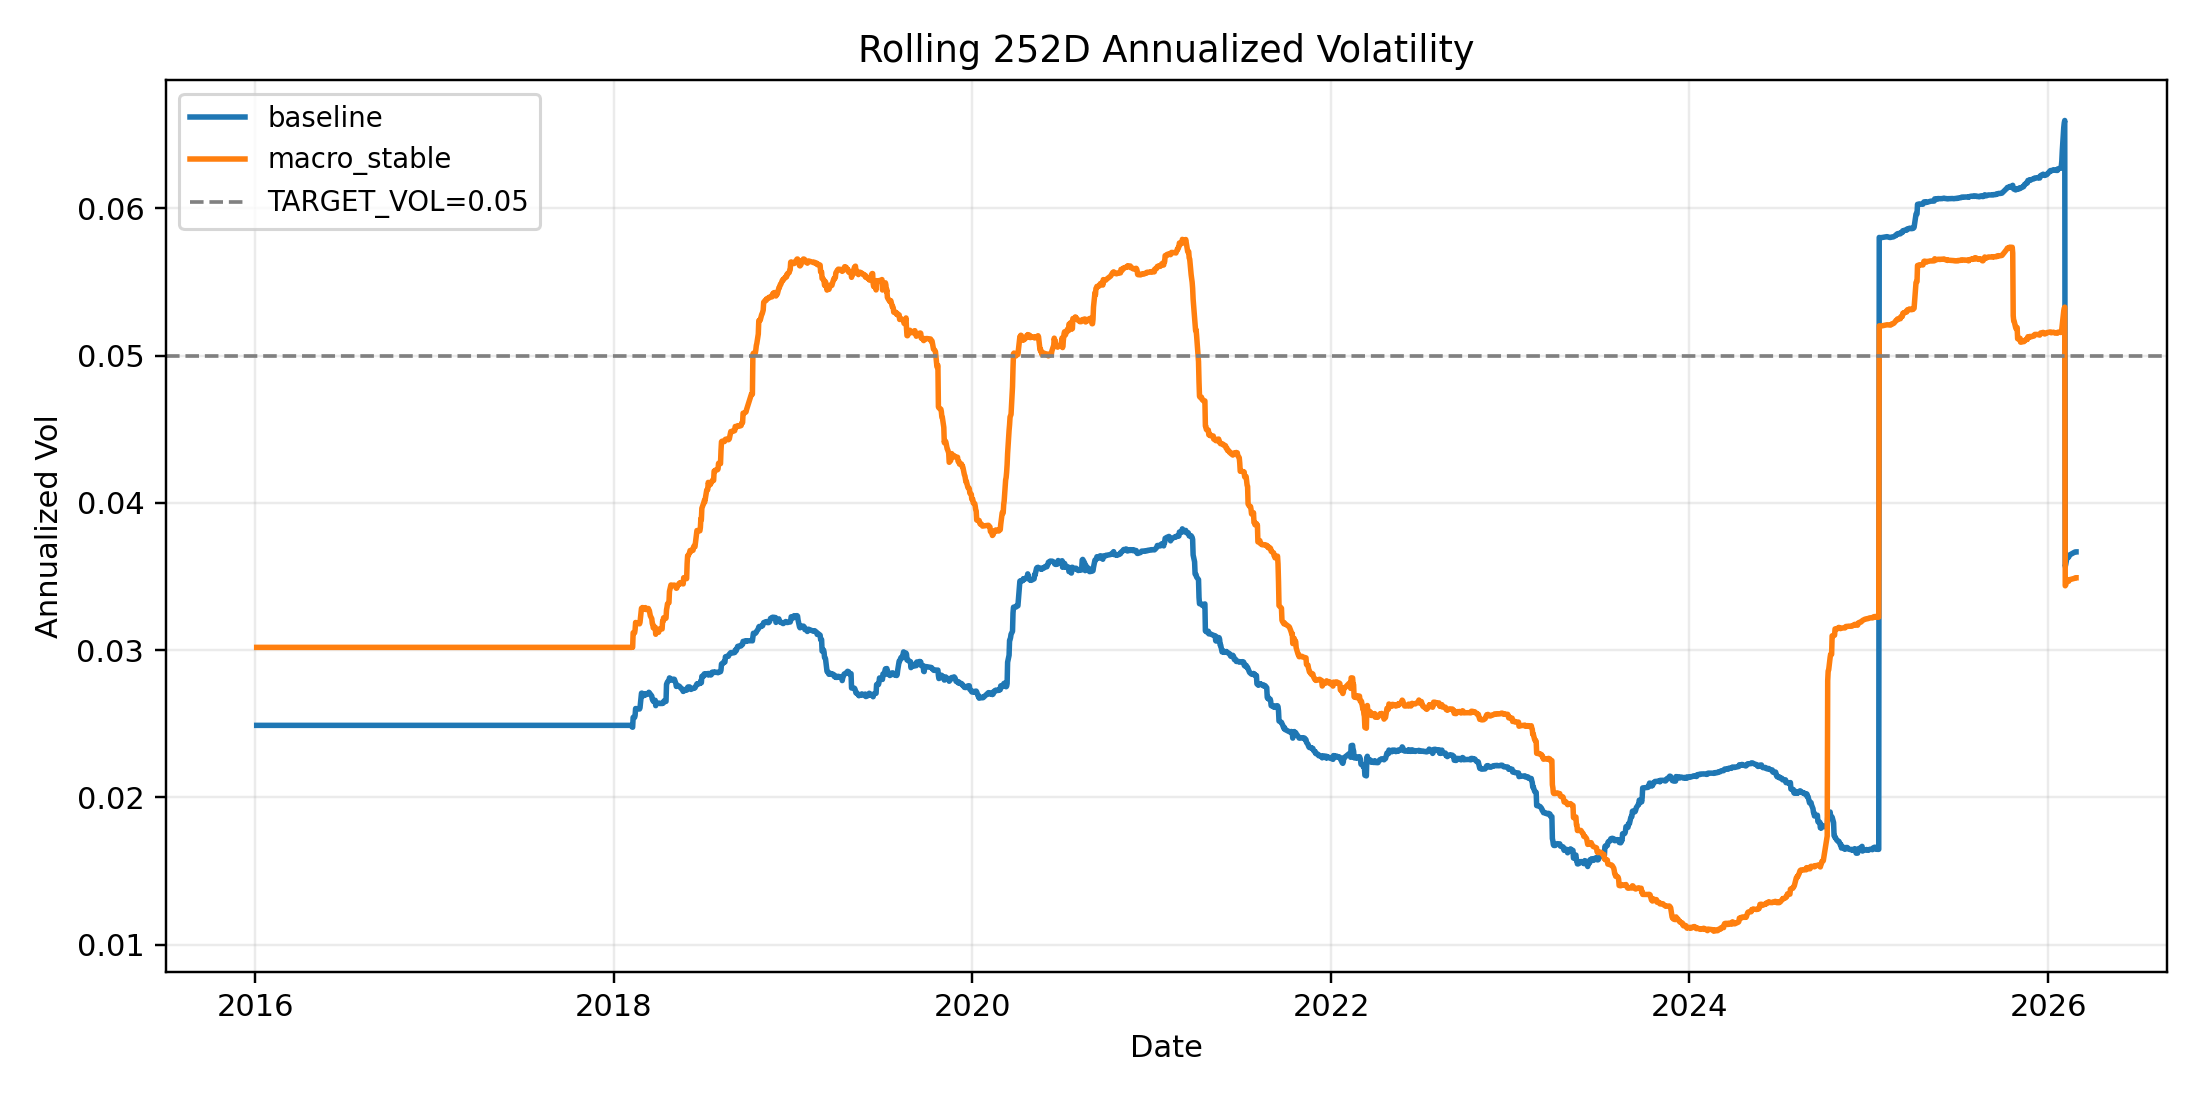
\includegraphics[width=0.88\textwidth]{showcase_output/figures/rolling_vol_252.png}
    \caption{252日滚动年化波动率}
\end{figure}

\subsection{权重结构与资产配置风格}

Baseline的权重配置更多由历史协方差决定，因此在某些时期容易向低波资产集中，尤其在债券类资产可得性较好、风险贡献更容易平衡时，出现较高单资产权重并不意外。Macro Stable则由于加入了单资产上限、单次权重变动限制和最低现金约束，权重结构整体更加均衡、更加机构化。

\begin{figure}[H]
    \centering
    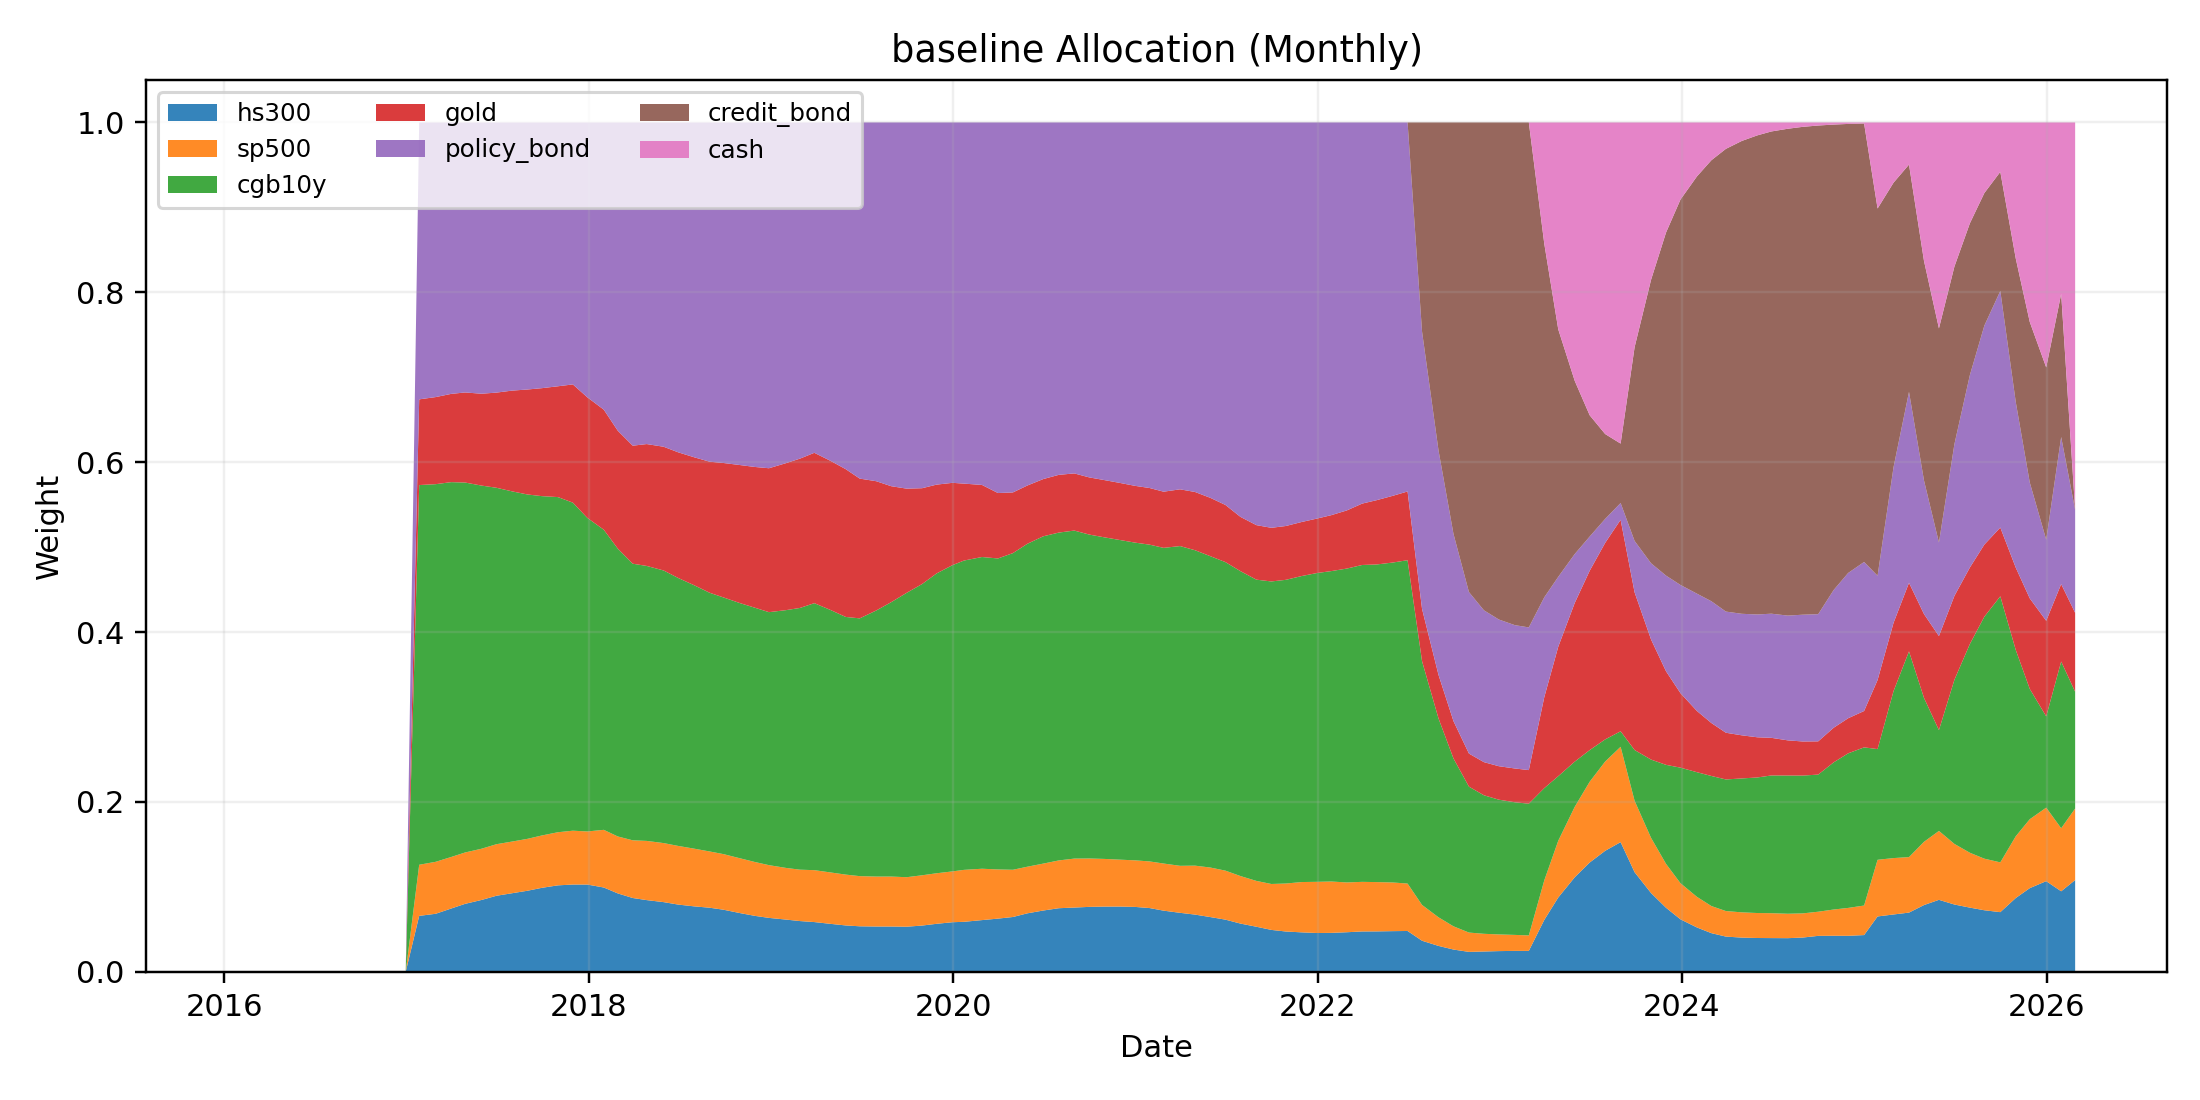
\includegraphics[width=0.88\textwidth]{showcase_output/figures/allocation_area_baseline.png}
    \caption{Baseline 月度资产配置结构}
\end{figure}

\begin{figure}[H]
    \centering
    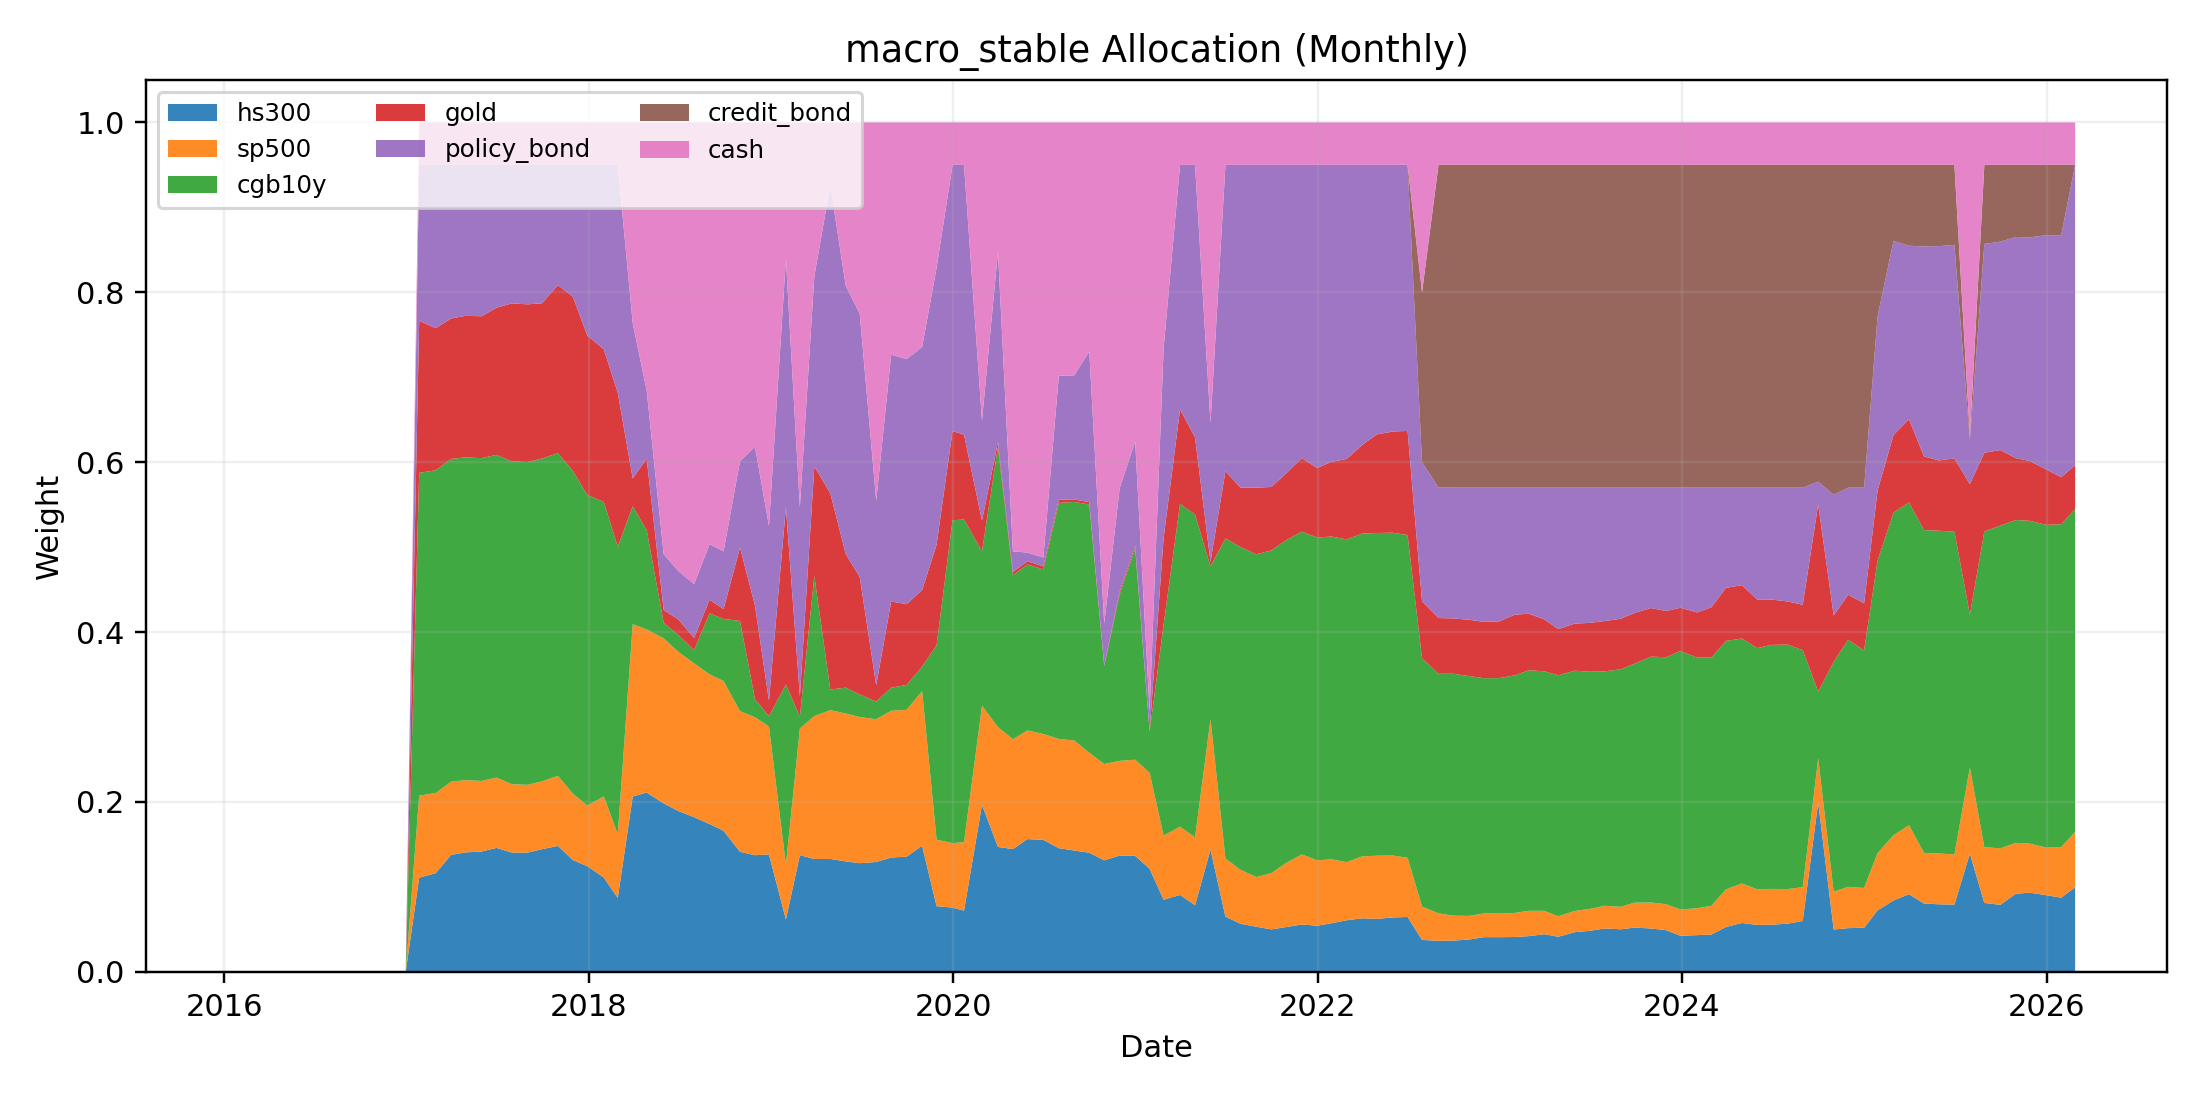
\includegraphics[width=0.88\textwidth]{showcase_output/figures/allocation_area_macro_stable.png}
    \caption{Macro Stable 月度资产配置结构}
\end{figure}

\subsection{现金权重与换手率}

现金比例的变化是本模型一个很值得讲的亮点。现金在这里不是“没配置出去的尾巴”，而是风险目标与风控约束共同作用后留下的主动缓冲层。Macro Stable的平均现金比例显著高于Baseline，这与其更低集中度、更强风险压缩能力相一致。

换手率图则反映出Macro Stable更频繁地根据状态与约束调整组合结构。摘要中也明确提示，应联动观察收益、波动、回撤、现金占比与换手率，避免只盯住单一指标得出结论。

\begin{figure}[H]
    \centering
    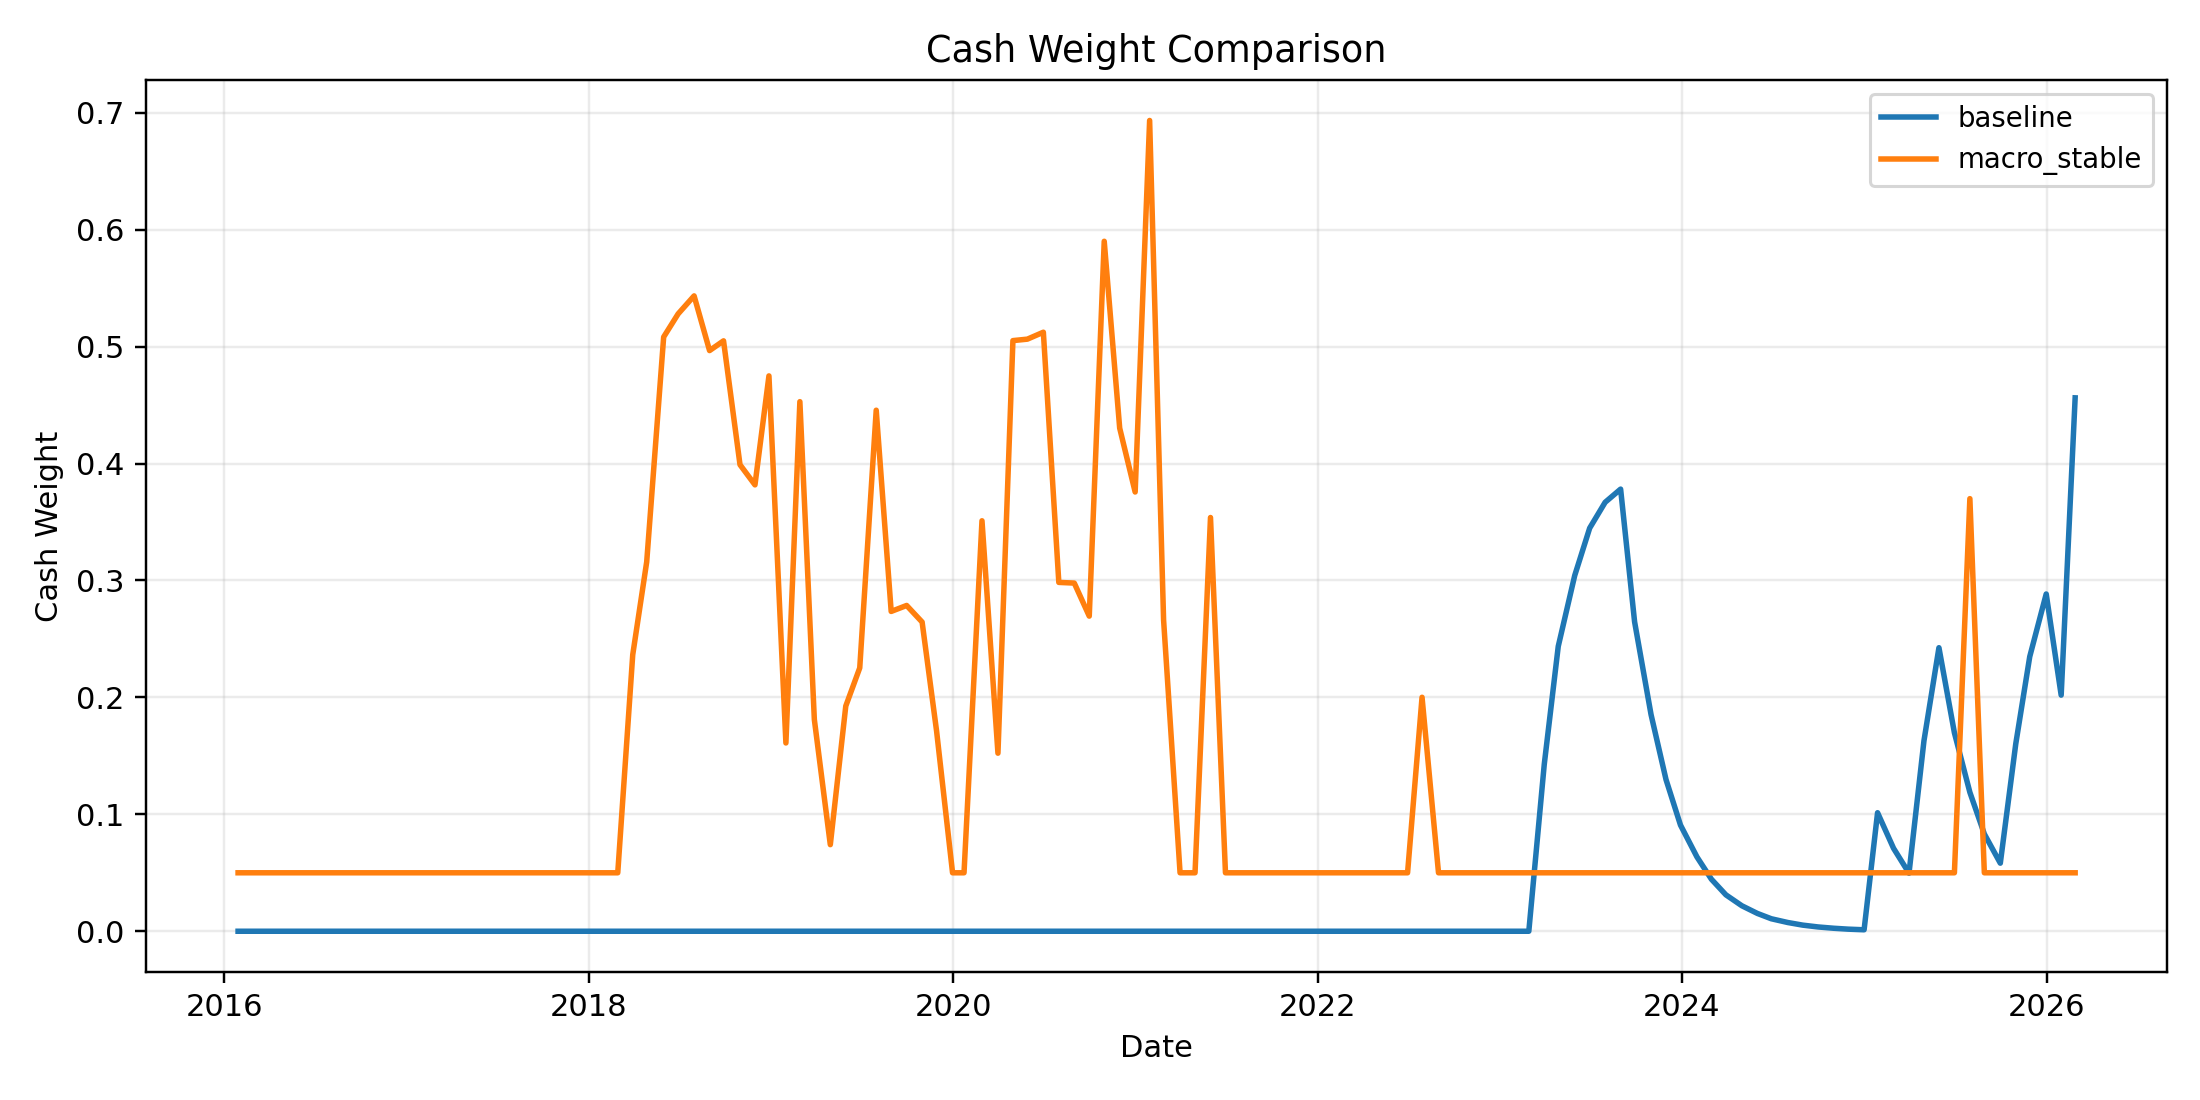
\includegraphics[width=0.88\textwidth]{showcase_output/figures/cash_weight_comparison.png}
    \caption{现金权重对比}
\end{figure}

\begin{figure}[H]
    \centering
    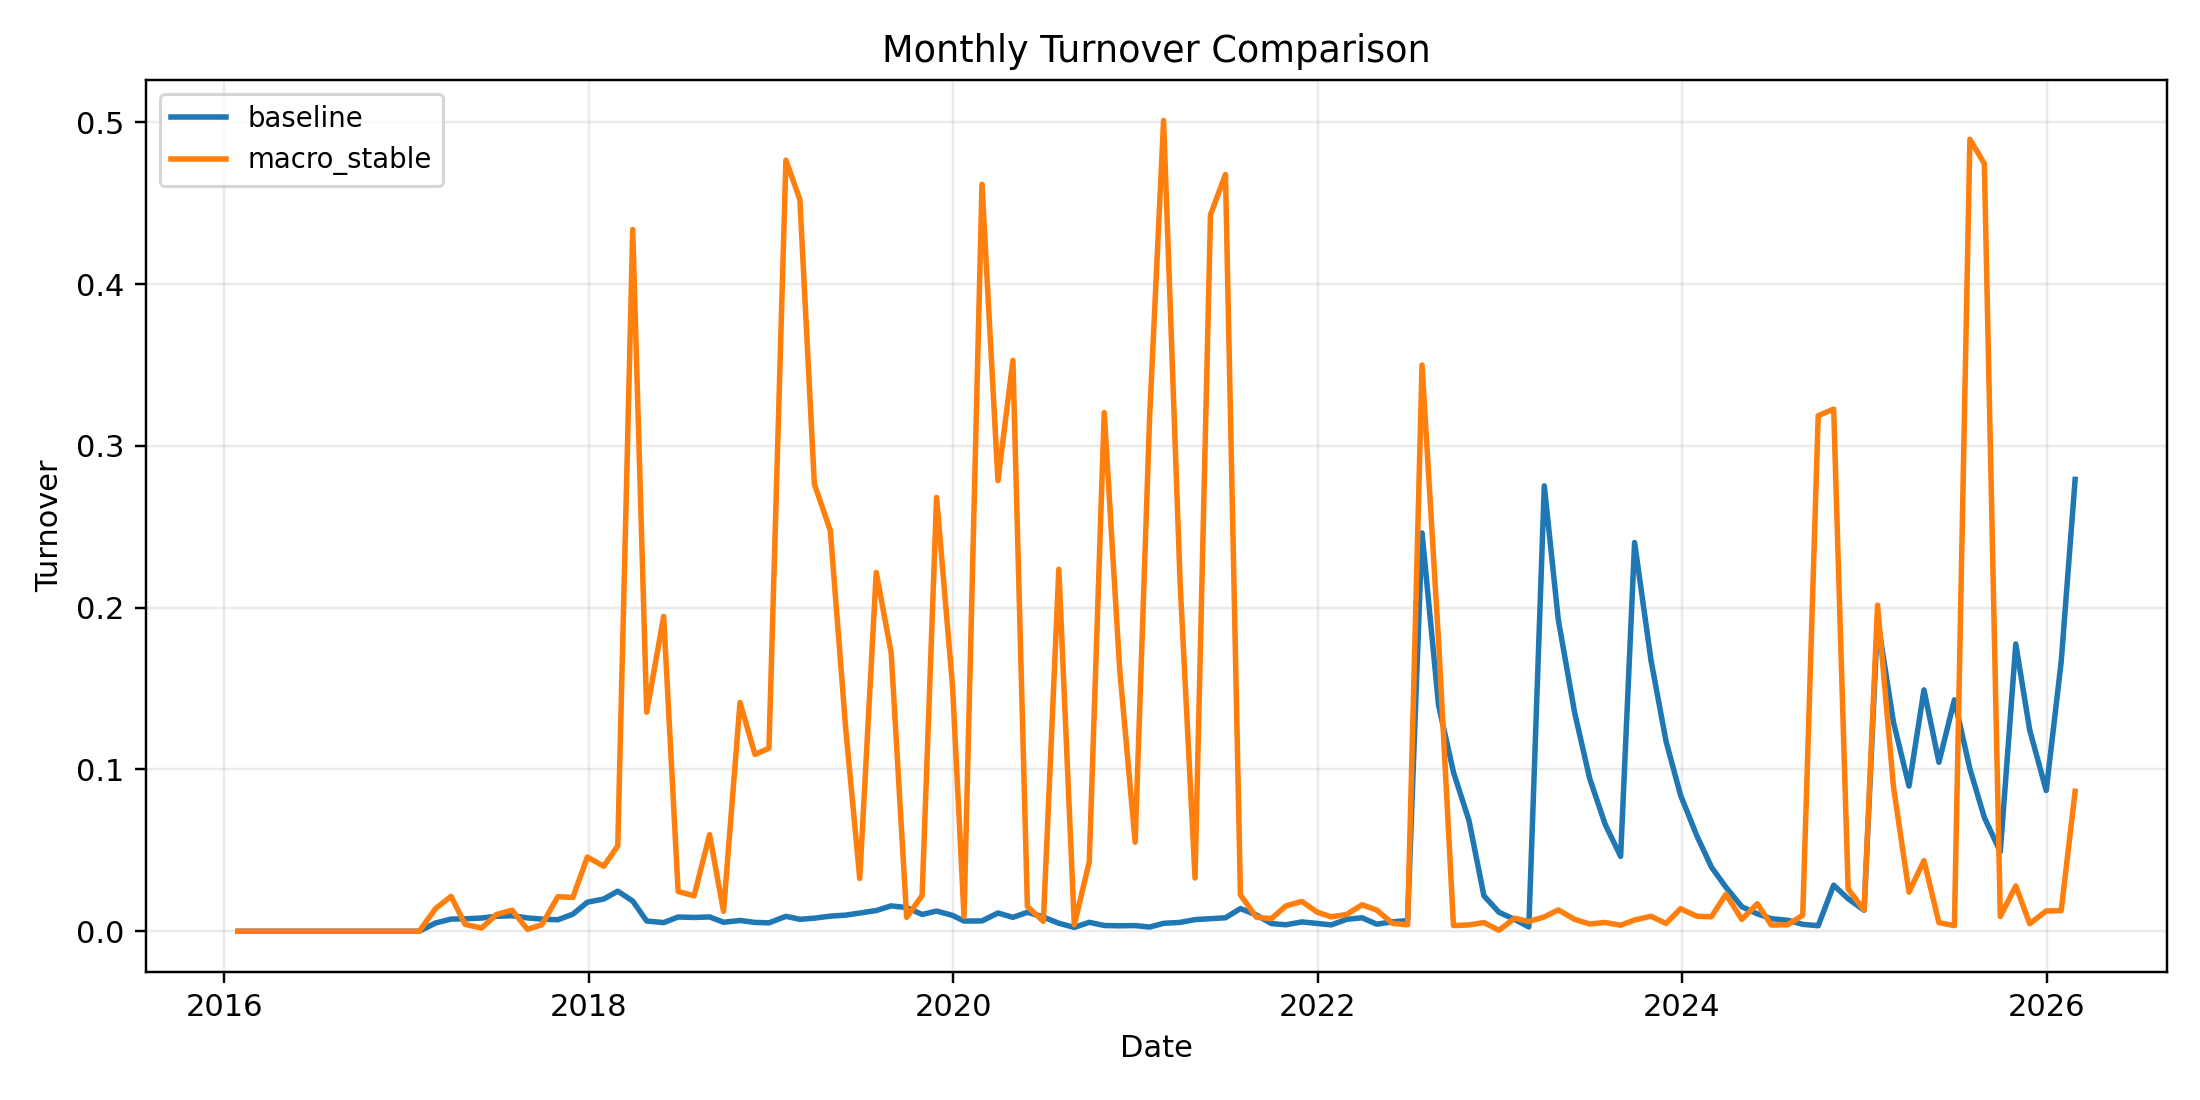
\includegraphics[width=0.88\textwidth]{showcase_output/figures/turnover_timeseries.png}
    \caption{月度换手率对比}
\end{figure}

% =========================
\section{为什么 Macro Stable 在验证段更占优}
% =========================

这是整篇报告里最值得认真解释的一部分。单看数字，很容易把结论粗暴地总结成“加了宏观因子后效果更好”。但真正更准确的说法应当是：

\begin{quote}
宏观信号通过重塑风险预算分配，使组合在状态切换时更早地改变风险暴露结构；而权重上限、调仓幅度限制、目标波动率缩放和最低现金约束，又让这种调整不会演化为失控的方向性下注。
\end{quote}

换句话说，Macro Stable在验证段胜出的原因，不是它“比Baseline更敢”，而是它“更会收，也更会放”。

具体来说，我认为有四点：

\begin{enumerate}[label=\arabic*)]
    \item \textbf{宏观预算替代了固定均分风险。}  
    Baseline默认各资产长期承担近似均等风险贡献，而Macro Stable允许在不同宏观状态下偏向更有利的资产类别。

    \item \textbf{约束链条更完整。}  
    宏观稳定版并不是单纯加一个宏观信号，而是把权重上限、单次变动限制、目标波动率与最低现金比例都嵌入执行顺序中。这让模型更像机构配置引擎，而不是课堂上的理想优化题。

    \item \textbf{验证期市场环境更适合状态响应。}  
    当市场处于明显的风格分化或宏观切换阶段时，固定风险预算往往不如条件风险预算更有适应性。

    \item \textbf{更高现金比例提高了组合弹性。}  
    平均现金仓位提升并不一定拖累组合，相反，在风险资产不稳定的阶段，它可能是组合回撤更浅、再进入更从容的重要来源。
\end{enumerate}

如果非要用一句更口语但又不失专业的话概括，那就是：Baseline像一个一直按照老规矩排兵布阵的将军，而Macro Stable则会先抬头看一眼天气、地形和风向，再决定兵力怎么分配。

% =========================
\section{模型局限与稳健性思考}
% =========================

尽管Macro Stable在验证段显示出较优表现，但本文仍有若干局限需要说明。

第一，信用债资产历史覆盖不完整，前段样本依赖指数、后段样本切换至ETF，可能导致部分阶段的风险特征不完全一致。

第二，宏观变量维度仍较简洁，目前主要围绕PMI、CPI与CN10Y构建状态识别。虽然解释性强，但也可能遗漏信用环境、流动性条件、美元因子或全球风险偏好等更复杂的信息。

第三，换手率在Macro Stable中明显更高，若未来引入真实交易成本、申赎冲击、税费与滑点，策略表现可能会被部分侵蚀。

第四，本文回测重点在于比较配置逻辑而非构造最优预测器，因此宏观信号仍偏规则驱动，未来可以进一步探索更系统的状态识别方法，例如隐马尔可夫模型、扩散指数或基于贝叶斯更新的宏观 regime 识别框架。

这些局限并不会推翻本文结论，但提醒我们：好的模型不是看起来没有缺点，而是知道自己的边界在哪里。

% =========================
\section{结论}
% =========================

本文围绕“宏观状态能否改善风险预算资产配置”这一问题，构建了Baseline风险平价模型与Macro Stable宏观驱动稳定版模型，并在统一的多资产ETF资产池中进行历史回测与验证比较。

研究表明，Baseline框架具备较强的简洁性与稳定性，但在面对宏观状态切换时，其固定风险预算机制存在响应不足的问题。Macro Stable则通过将宏观信号嵌入风险预算分配，同时辅以单资产上限、单次调仓限制、目标波动率缩放与最低现金比例约束，使得组合在状态切换期间更具适应性和执行纪律。

从实证结果看，Macro Stable在回测段收益略高但承担了更高波动与更深回撤，而在验证段则同时实现了更高收益、更低波动和更浅回撤，Sharpe比率也显著优于Baseline。与此同时，Macro Stable具有更高的现金比例、更低的最大单资产集中度，以及更高的换手率。这说明该模型并非无代价地“变好”，而是在收益、风险、分散度和交易频率之间做出了更偏机构化的重新平衡。

最终，本文的结论并不是“宏观因子万能”，而是：

\begin{quote}
在风险预算框架中引入宏观状态，不应理解为用宏观去替代风险平价，而应理解为让风险平价在不同经济环境下拥有条件化表达能力。
\end{quote}

这也是我认为本次课题最有价值的地方。它不是在旧模型上贴一层宏观标签，而是把宏观信息真正嵌进了配置逻辑的骨架里。

% =========================
\section*{附录A：核心指标汇总}
\addcontentsline{toc}{section}{附录A：核心指标汇总}
% =========================

\begin{table}[H]
\centering
\caption{Baseline 与 Macro Stable 核心绩效指标对比}
\begin{threeparttable}
\begin{tabular}{lcc}
\toprule
指标 & Baseline & Macro Stable \\
\midrule
\multicolumn{3}{c}{\textbf{回测段（2018--2023）}} \\
年化收益率 & 4.25\% & 4.54\% \\
年化波动率 & 2.78\% & 3.99\% \\
Sharpe比率 & 1.529 & 1.137 \\
最大回撤 & -3.27\% & -6.12\% \\
Calmar比率 & 1.298 & 0.742 \\
\midrule
\multicolumn{3}{c}{\textbf{验证段（2024--2025）}} \\
年化收益率 & 5.11\% & 6.77\% \\
年化波动率 & 4.71\% & 4.44\% \\
Sharpe比率 & 1.086 & 1.527 \\
最大回撤 & -6.65\% & -5.47\% \\
Calmar比率 & 0.769 & 1.239 \\
\midrule
平均现金比例 & 4.60\% & 15.39\% \\
最大单资产权重 & 59.46\% & 38.83\% \\
最大单次权重变化 & 24.62\% & 20.16\% \\
月度平均换手率 & 3.82\% & 8.92\% \\
\bottomrule
\end{tabular}
\begin{tablenotes}
\footnotesize
\item 注：上述指标来自展示摘要自动输出结果。
\end{tablenotes}
\end{threeparttable}
\end{table}

\noindent 数据来源与指标结果依据项目自动输出摘要整理。

% =========================
\section*{附录B：年度表现图}
\addcontentsline{toc}{section}{附录B：年度表现图}
% =========================

\begin{figure}[H]
    \centering
    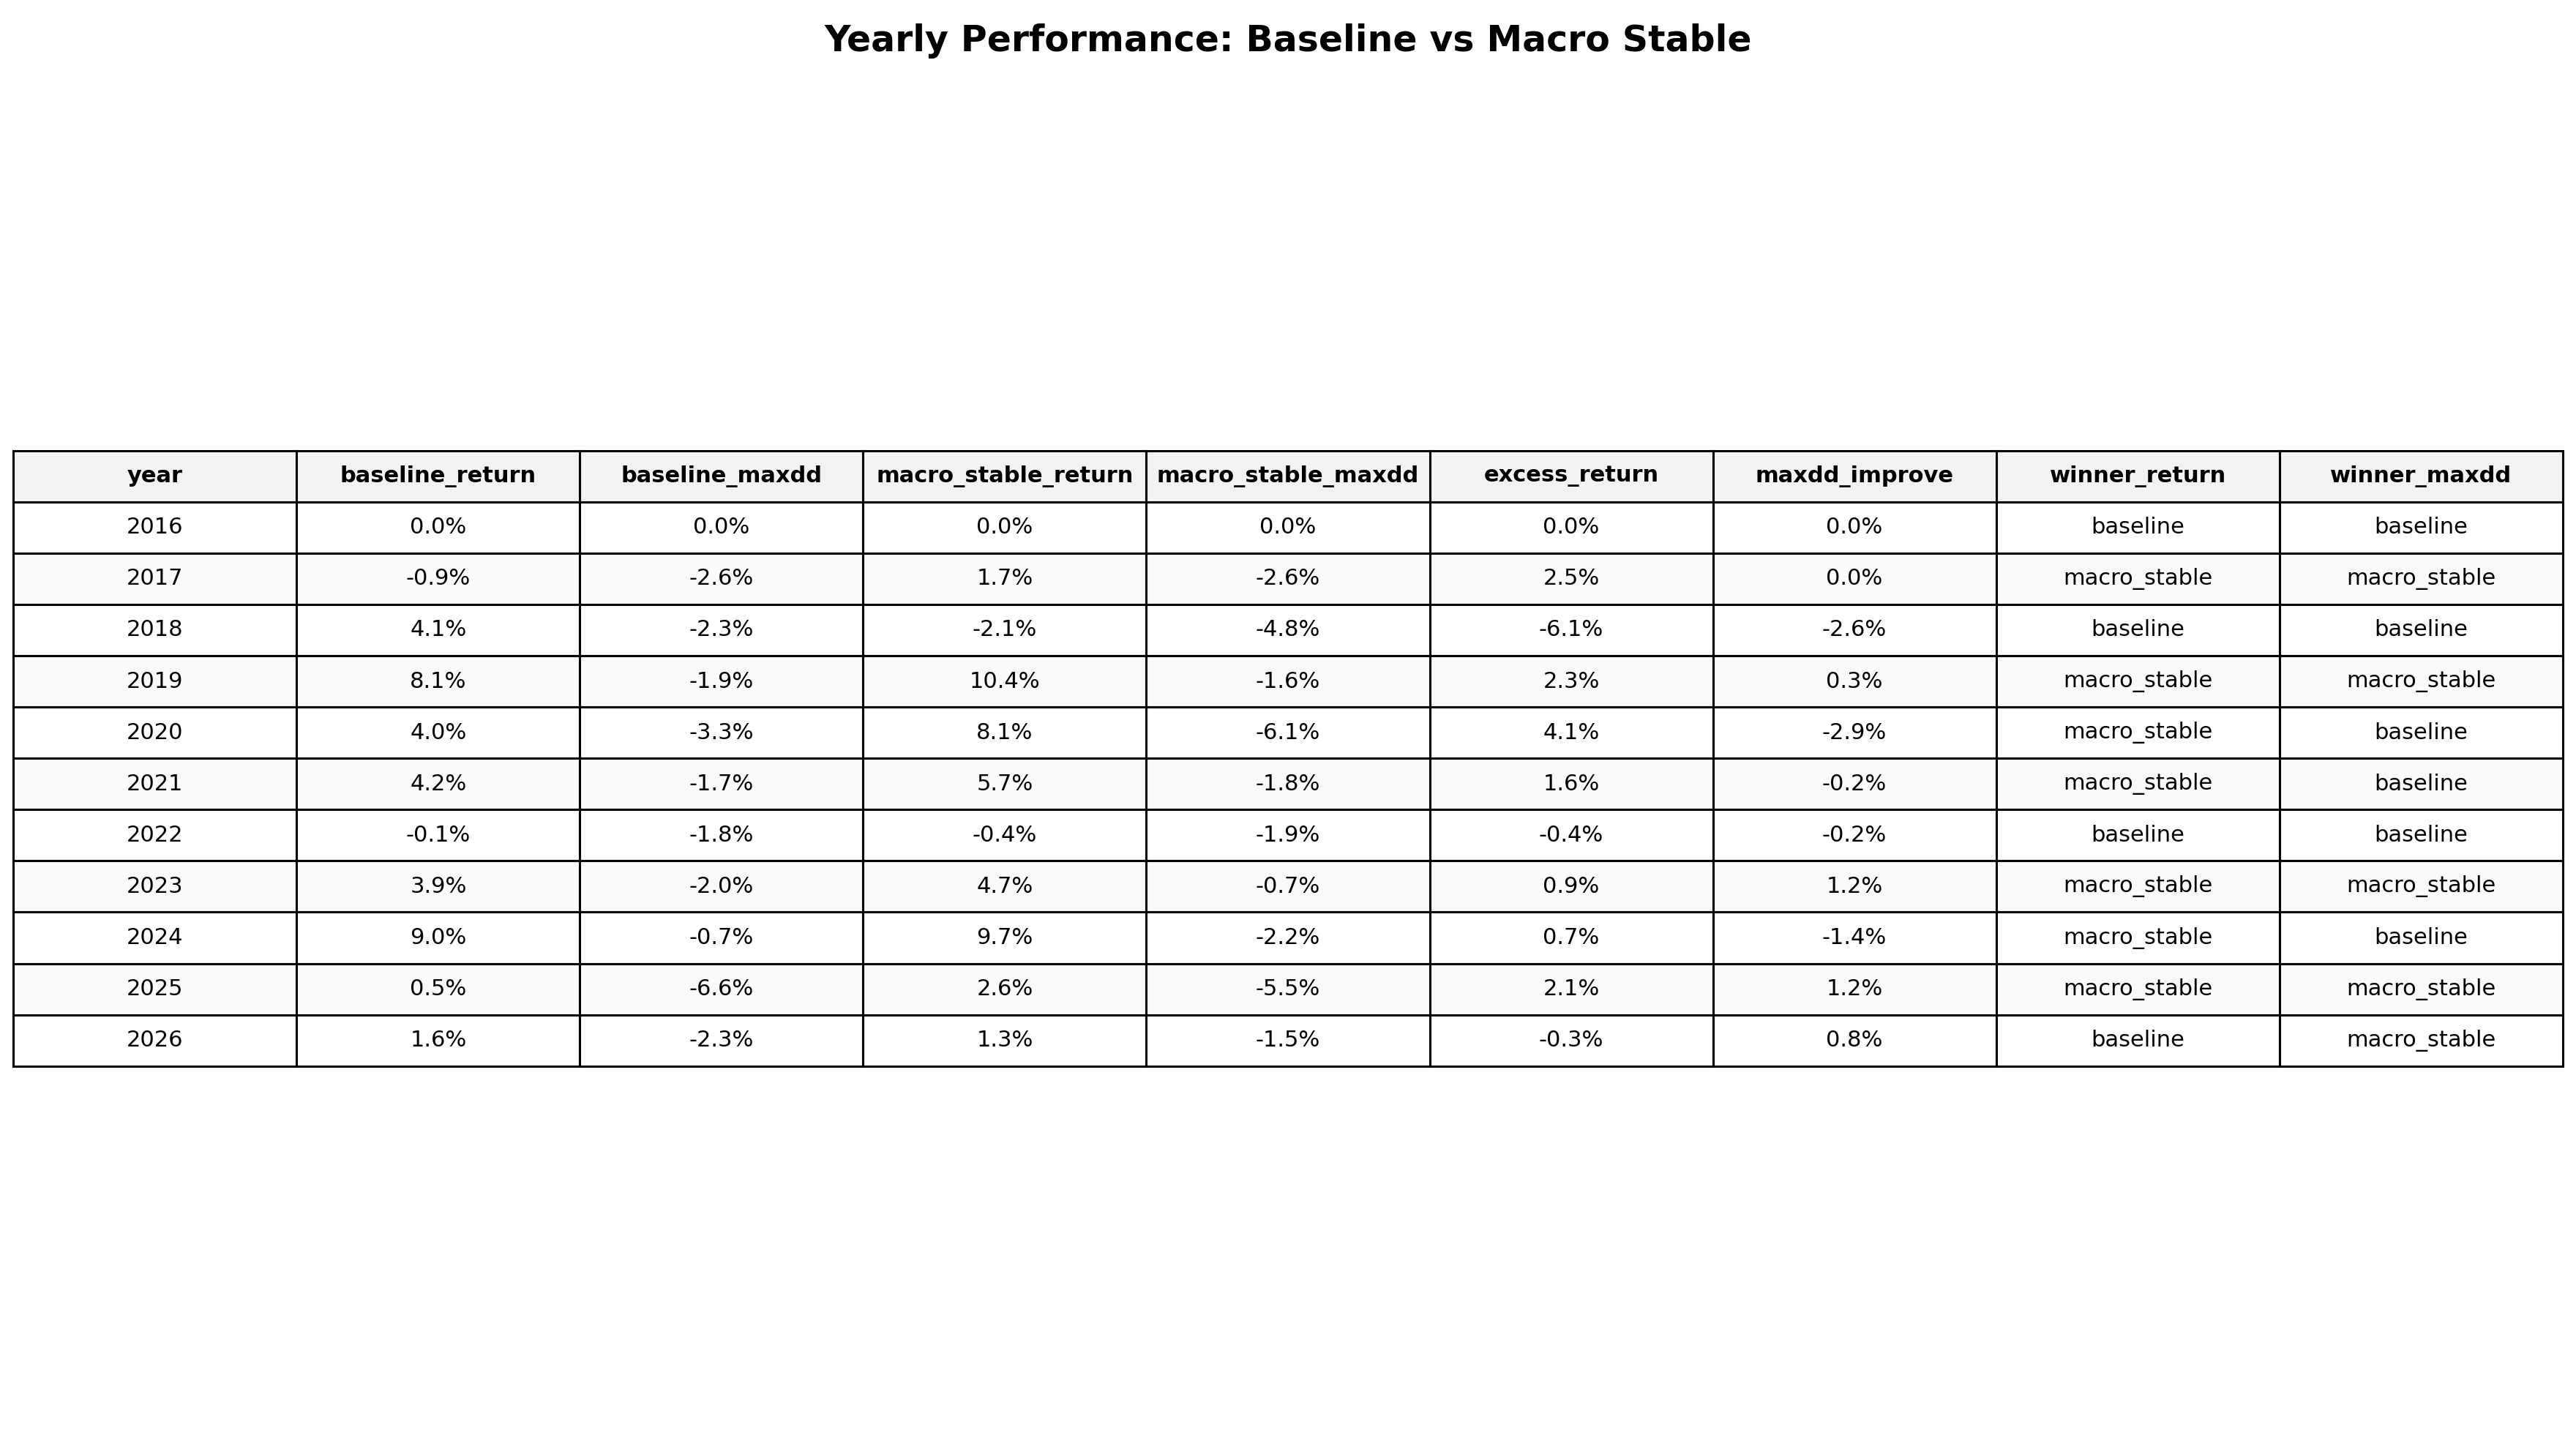
\includegraphics[width=0.95\textwidth]{showcase_output/figures/perf_by_year.png}
    \caption{年度收益与最大回撤对比}
\end{figure}

% =========================
\section*{附录C：可选参考文献模板}
\addcontentsline{toc}{section}{附录C：可选参考文献模板}
% =========================

\begin{thebibliography}{99}

\bibitem{markowitz1952}
Markowitz, H. (1952).
\newblock Portfolio Selection.
\newblock \emph{The Journal of Finance}, 7(1), 77--91.

\bibitem{qian2005}
Qian, E. (2005).
\newblock Risk Parity Portfolios: Efficient Portfolios Through True Diversification.
\newblock \emph{PanAgora Asset Management Research Paper}.

\bibitem{maillard2010}
Maillard, S., Roncalli, T., \& Te{\"i}letche, J. (2010).
\newblock The Properties of Equally Weighted Risk Contribution Portfolios.
\newblock \emph{The Journal of Portfolio Management}, 36(4), 60--70.

\bibitem{citic2025}
\textbf{中信证券研究部.} (2025).
\newblock 多资产ETF的海外经验与国内展望.
\newblock \emph{资产配置专题系列之三十八}.

\end{thebibliography}

\end{document}